\documentclass[12pt]{article}
\usepackage{graphicx}
\usepackage{epstopdf}
\usepackage{booktabs}
\usepackage[table]{xcolor}
\usepackage{float}
\usepackage{caption}
\usepackage{hyperref}
\usepackage{adjustbox}
\usepackage{amsmath}
\usepackage{listings}
\usepackage[document]{ragged2e}
\usepackage{titling}
\usepackage{lipsum}

\author{Assignment 0 \\Vaishali Pal \\ 201407665}
\title{Computer Vision Assignment Report}
\date{\today}


\preauthor{\begin{flushright}\large} % makes author flush right
\postauthor{\end{flushright}}

\begin{document}
  \maketitle
  
\section{Introduction}
The purpose of this assignment is to be familiar with openCV library and to perform basic operations like reading and writing images and videos. Further, a composite of two videos is created using chroma keying technique. OpenCV 2.4.11 has been used for the experiments and the programs are written in c++ and compiled with c++11 compiler. 

\section{Conversion of a Video to Images}
A video comprises of a sequence of images called frames which forms a moving picture. OpenCV allows for a video to be read by reading its constituent frames through the VideoCapture class. It is a class for video capturing from video files, image sequences or cameras.  The constructor
\begin{verbatim} VideoCapture (const String &filename)
\end{verbatim} opens the video file and initializes the VideoCapture object for reading the video stream from the specified file.
\begin{verbatim} 
bool IsOpened()
\end{verbatim} checks whether the previous call to VideoCapture constructor is successful and returns \texttt{true} if successful, else returns \texttt{false}. The function \begin{verbatim}bool imwrite(const string& filename, InputArray img, 
             const vector<int>& params=vector<int>())\end{verbatim} saves an image to a specified file.
\subsection{Code} 
\begin{lstlisting}[language=c++]
#include<opencv2/core/core.hpp>
#include<opencv2/highgui/highgui.hpp>
#include<iostream>
#include<string>

using namespace cv;
using namespace std;

int main(int argc, char** argv)
{
         //name of video file
         String videoPath("Spirit_ Stallion of the Cimarron.mp4");
         if (argc == 2)
                 videoPath = argv[1];

         //object to capture video 
         VideoCapture cap(videoPath);
         if (!cap.isOpened()) {
                 cerr << "Error: could not load video\n";
                 return -1;
         }

         //Capture successive frames from video object
         Mat frame;
         int num = 1;
         while(true) {
                 cap >> frame;
                 if(!frame.data)
                         break;

                 //write frame to file
              string filename = "me/frame" +  to_string(num++) + ".jpg";
                 imwrite(filename, frame);
         }
   return 0;
}

\end{lstlisting}

\subsection{Input}
The input to the program was a 2:10 minute video of an animation. The video can be found in the following link \url{https://www.youtube.com/watch?v=Zlm4QYeysgE}

\subsection{Output}
The output is the constituent frames of the video.
The video frames can be viewed at \url{https://www.dropbox.com/sh/7zan9vye5w1wz8q/AAAJ8yzs1mNQIPngq9rgZna2a?dl=0}
The first few frames of the video are as follows:


\begin{figure}[htp]
\centering
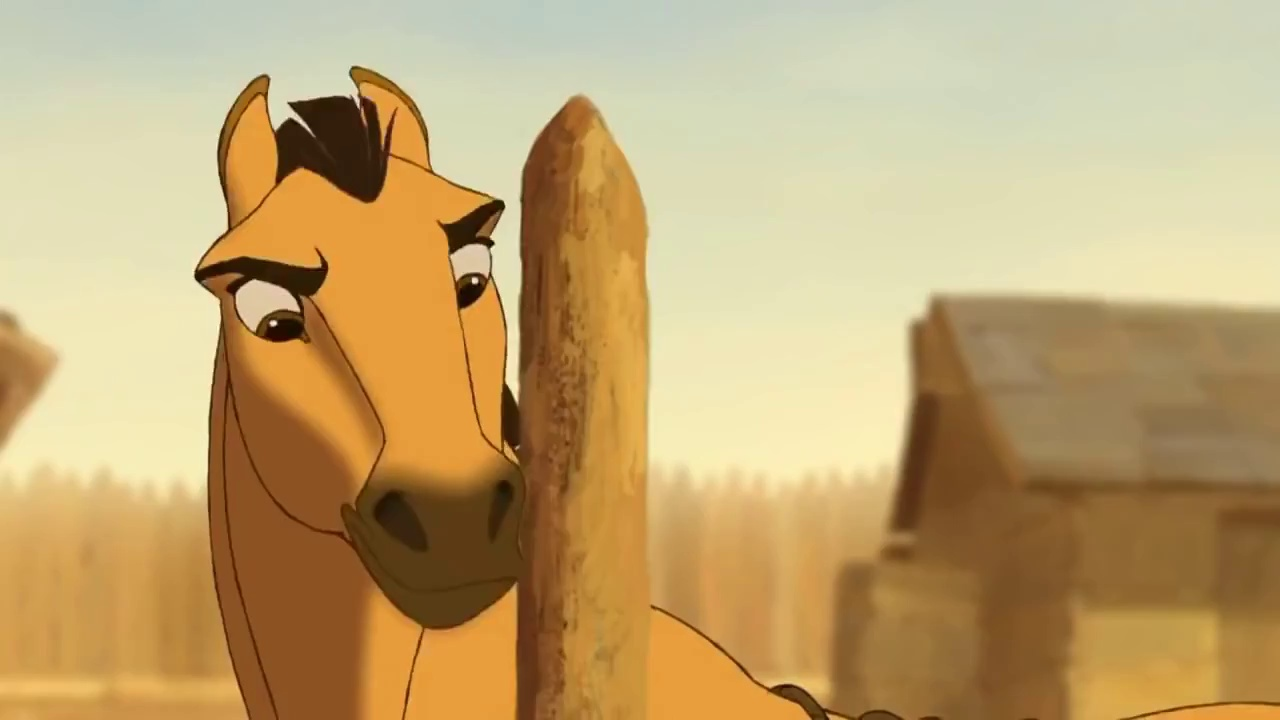
\includegraphics[width=.33\textwidth]{videoFrames/frame1.jpg}\hfill
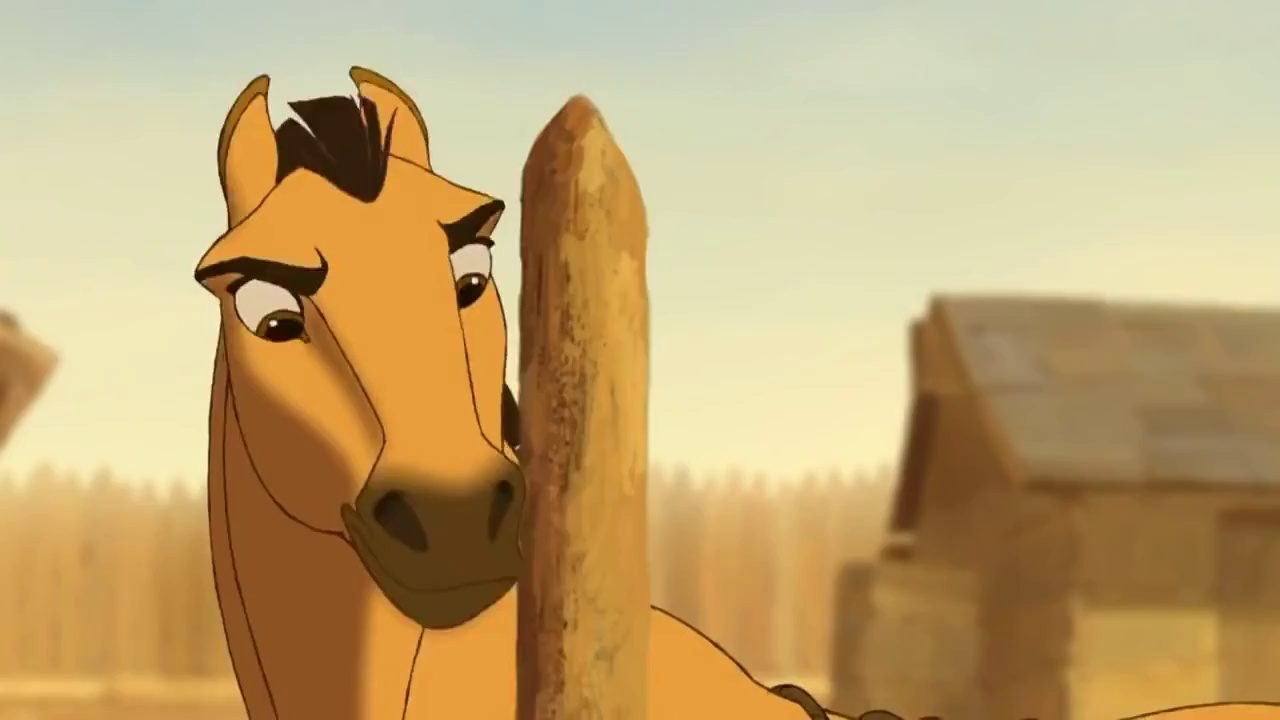
\includegraphics[width=.33\textwidth]{{videoFrames/frame2.jpg}}\hfill
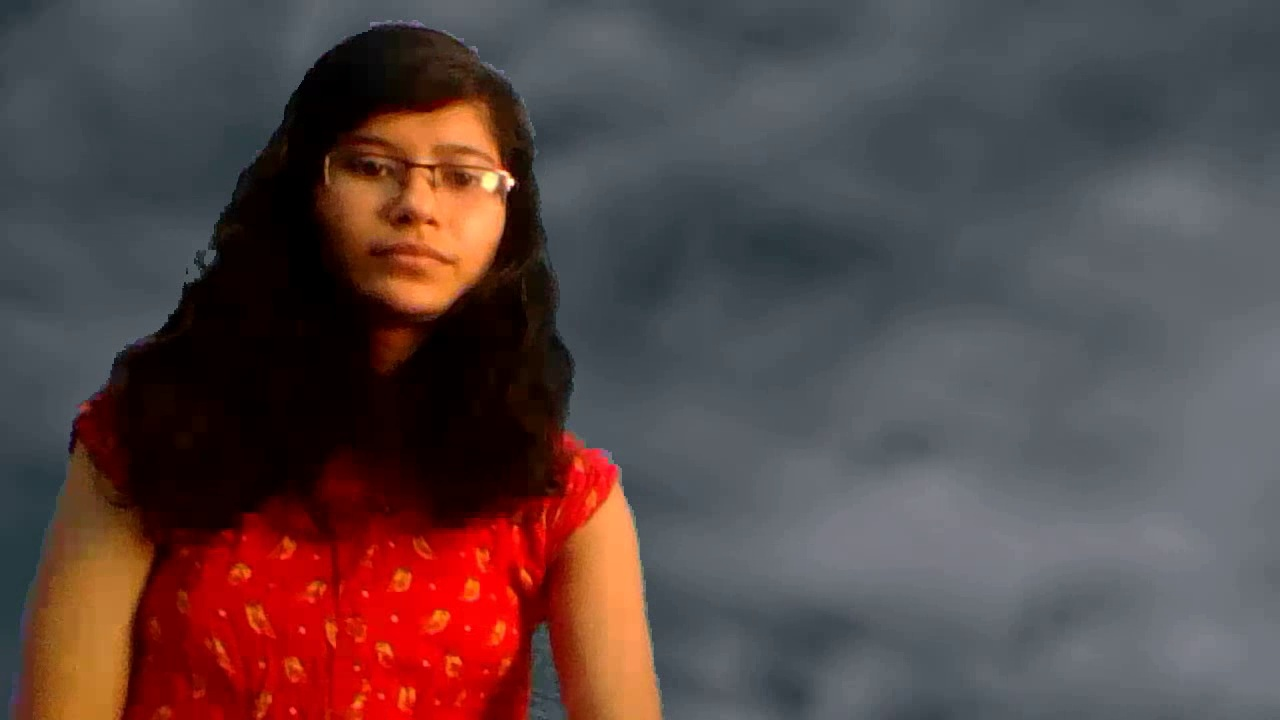
\includegraphics[width=.33\textwidth]{{videoFrames/frame3.jpg}}
\end{figure}
\label{figure1}

\begin{figure}[htp]
\centering
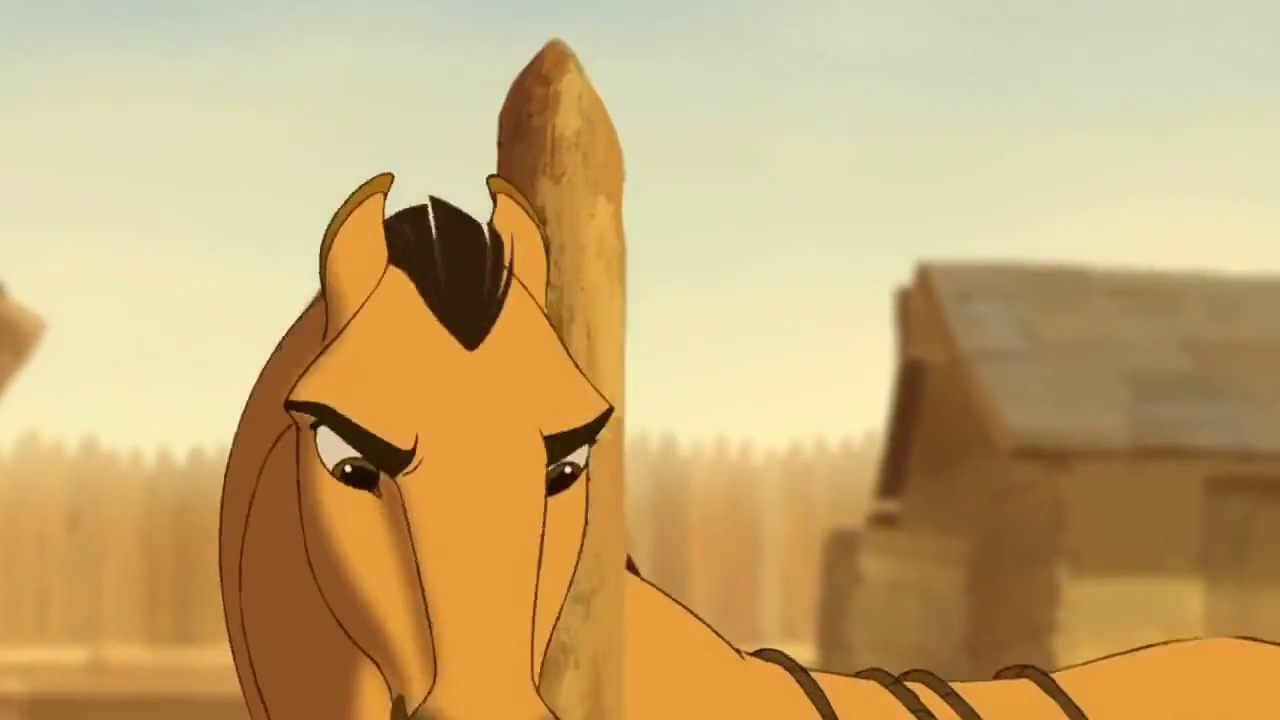
\includegraphics[width=.33\textwidth]{videoFrames/frame4.jpg}\hfill
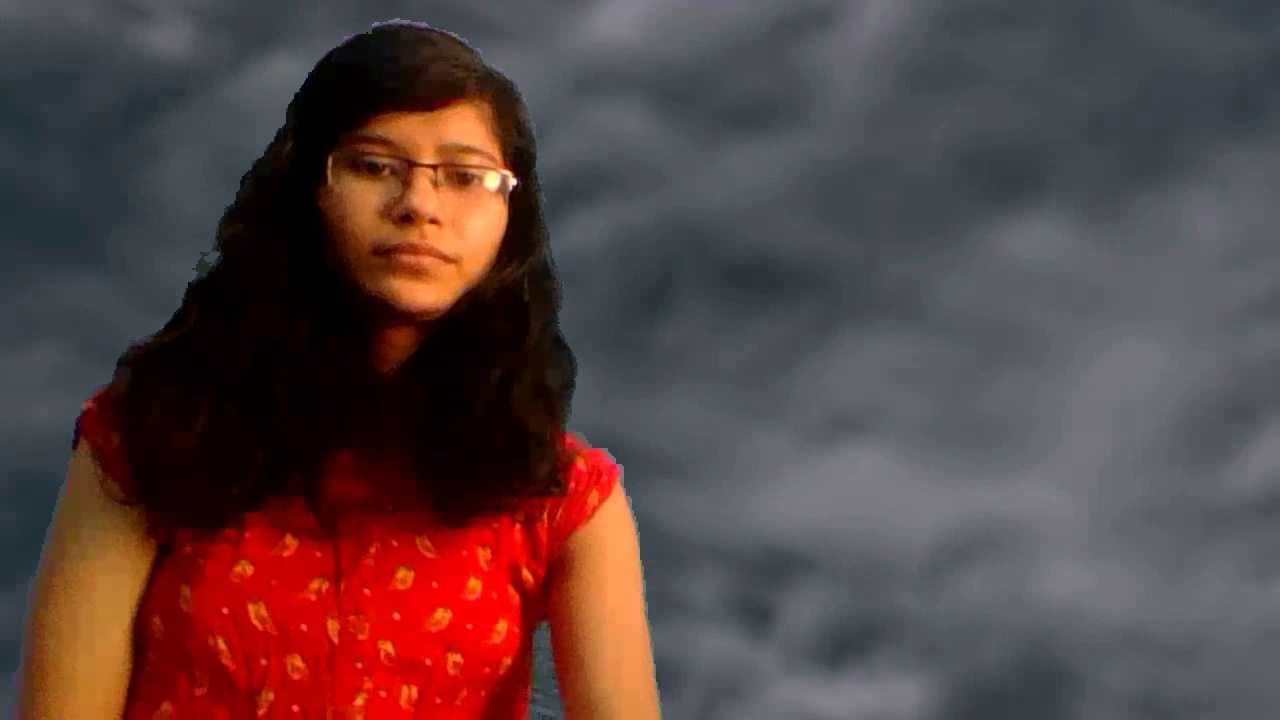
\includegraphics[width=.33\textwidth]{{videoFrames/frame5.jpg}}\hfill
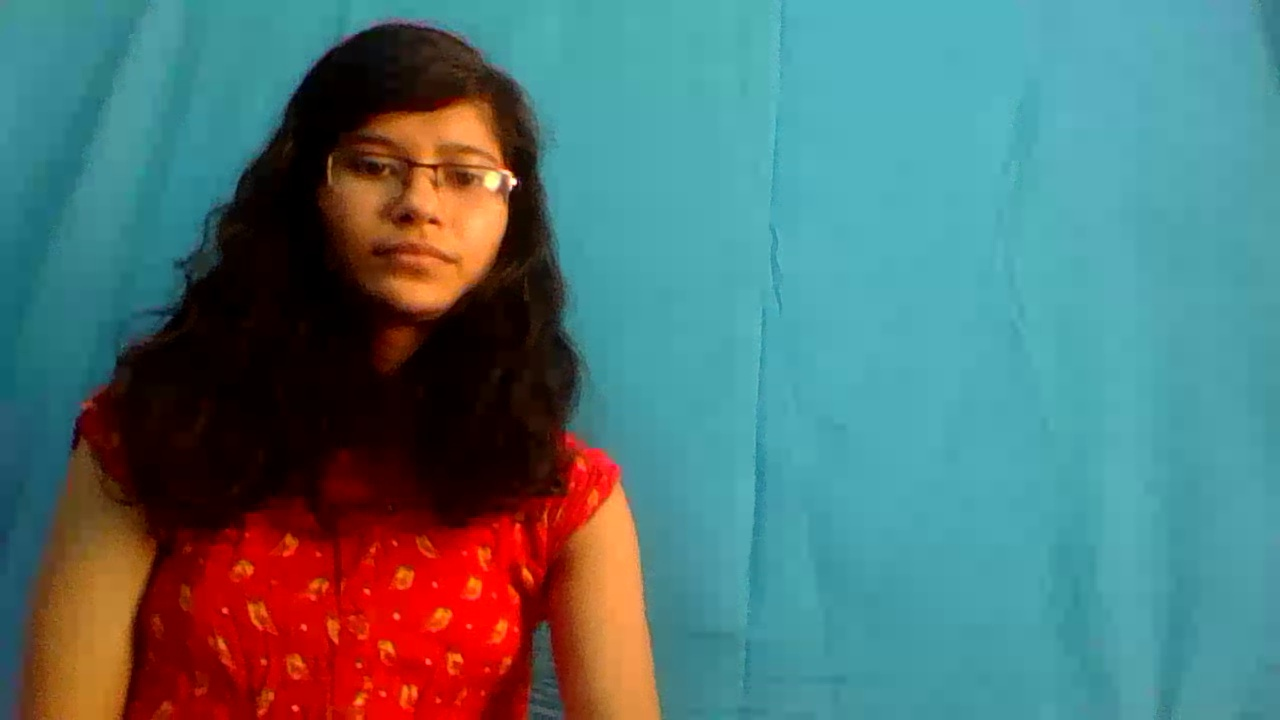
\includegraphics[width=.33\textwidth]{{videoFrames/frame6.jpg}}
\end{figure}

\begin{figure}[htp]
\centering
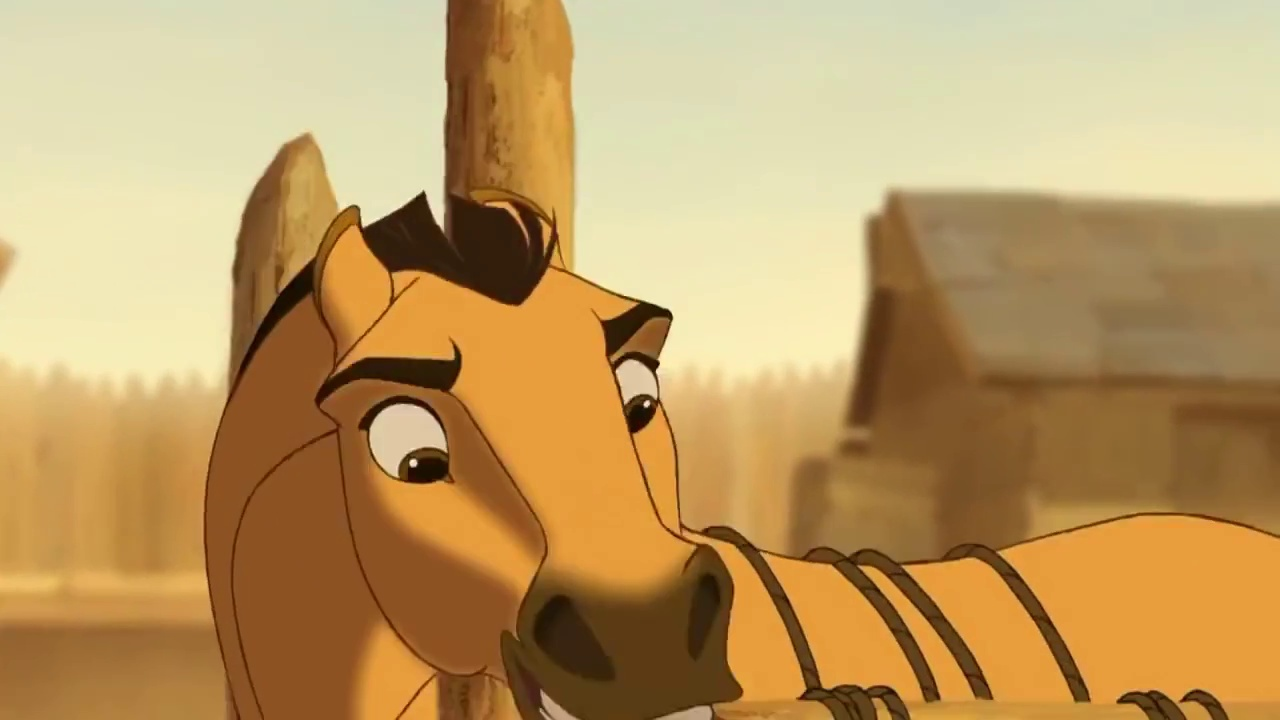
\includegraphics[width=.33\textwidth]{videoFrames/frame7.jpg}\hfill
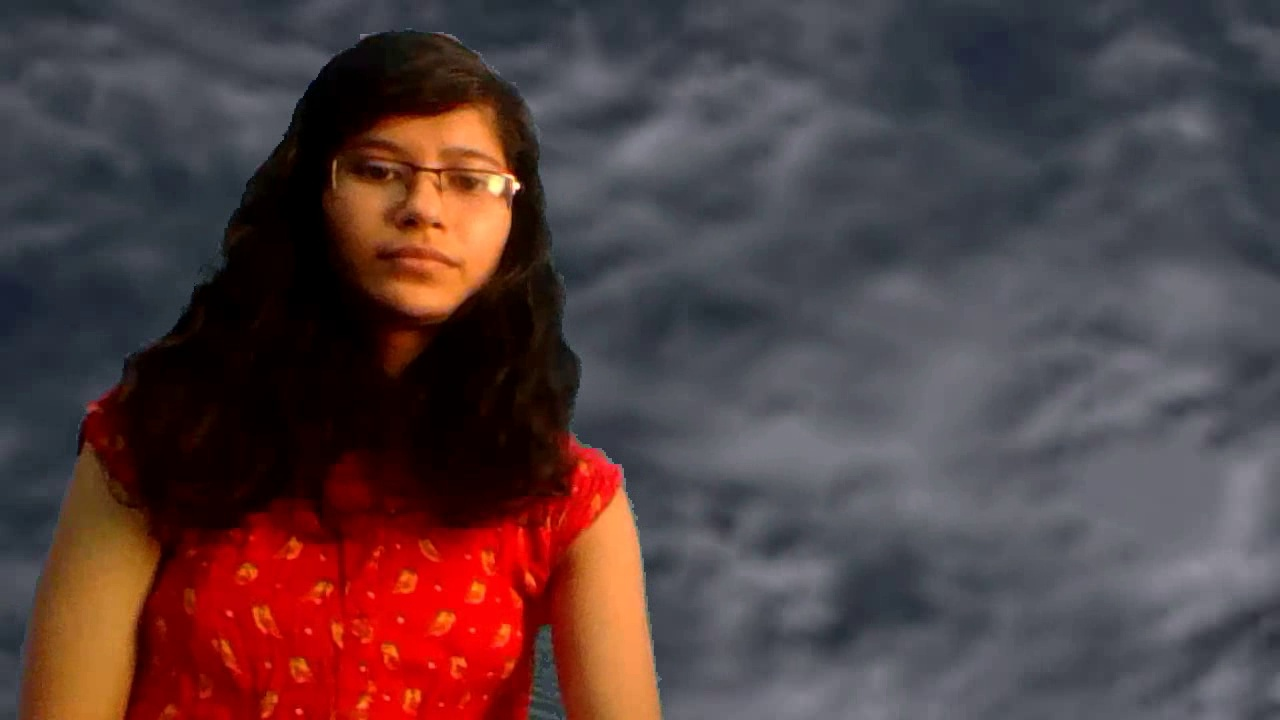
\includegraphics[width=.33\textwidth]{{videoFrames/frame8.jpg}}\hfill
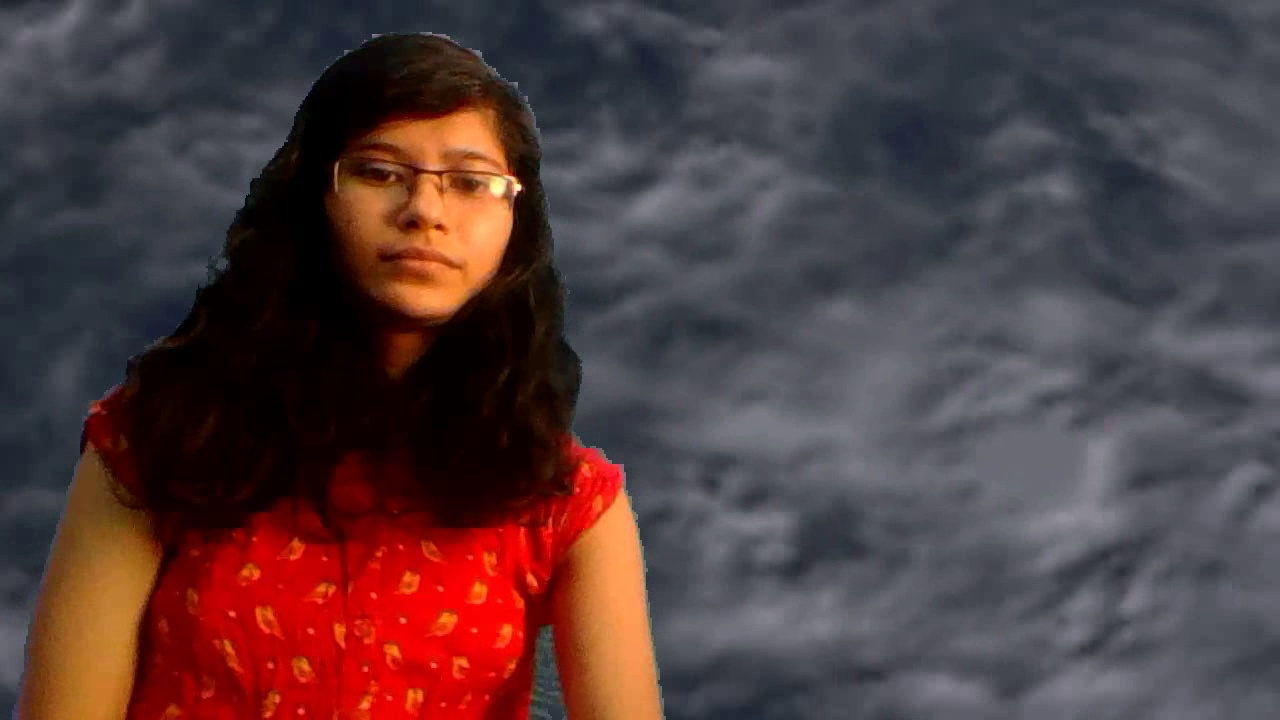
\includegraphics[width=.33\textwidth]{{videoFrames/frame9.jpg}}
\end{figure}

\begin{figure}[htp]
\centering
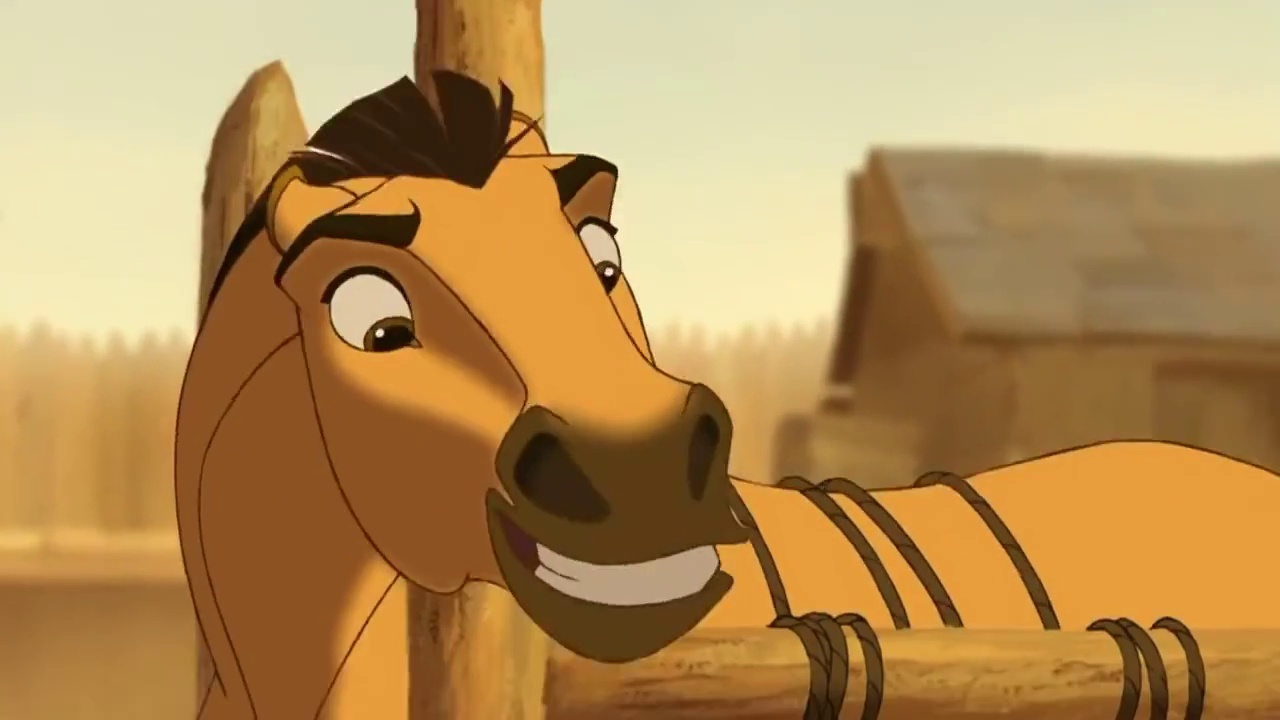
\includegraphics[width=.33\textwidth]{videoFrames/frame10.jpg}\hfill
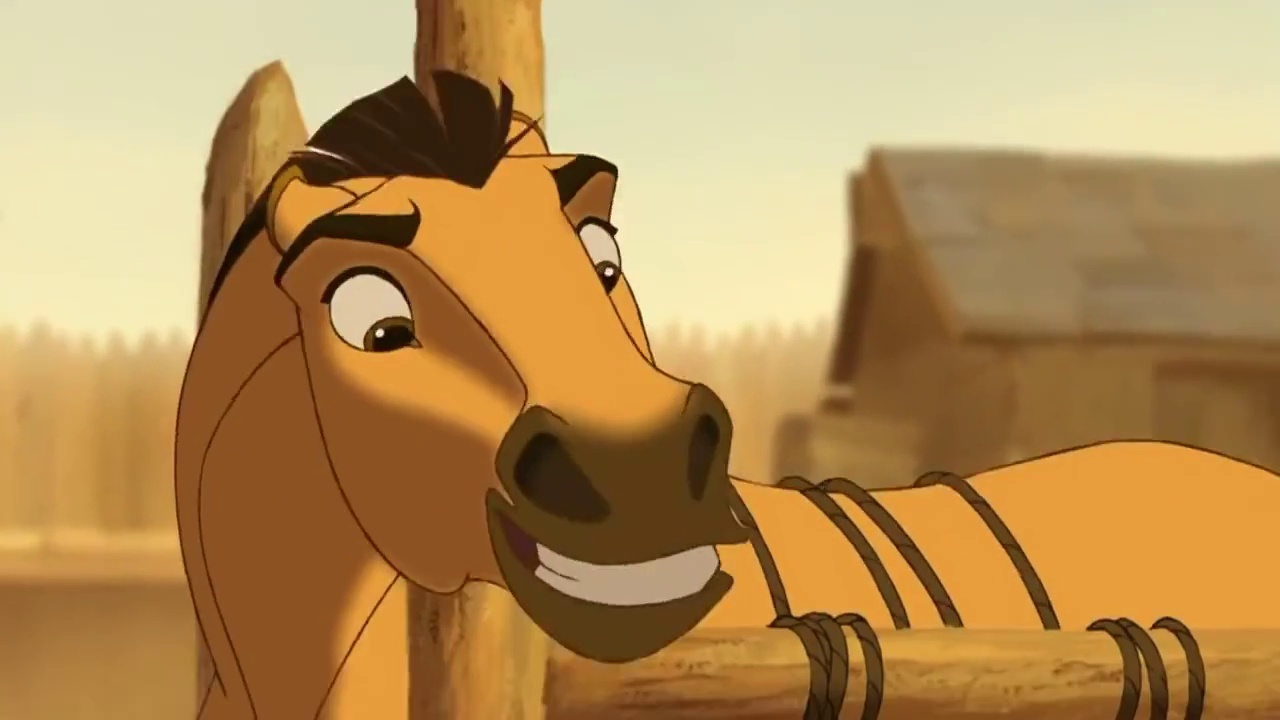
\includegraphics[width=.33\textwidth]{{videoFrames/frame11.jpg}}\hfill
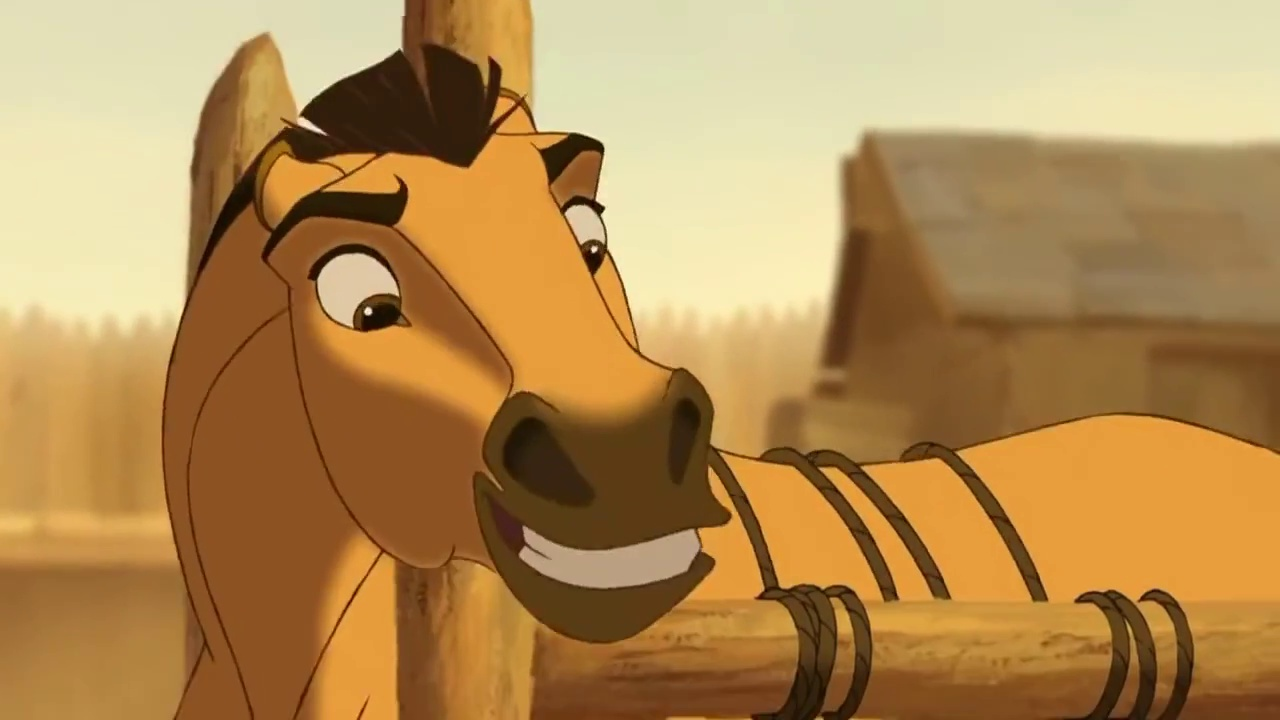
\includegraphics[width=.33\textwidth]{{videoFrames/frame12.jpg}}
\end{figure}

\begin{figure}[htp]
\centering
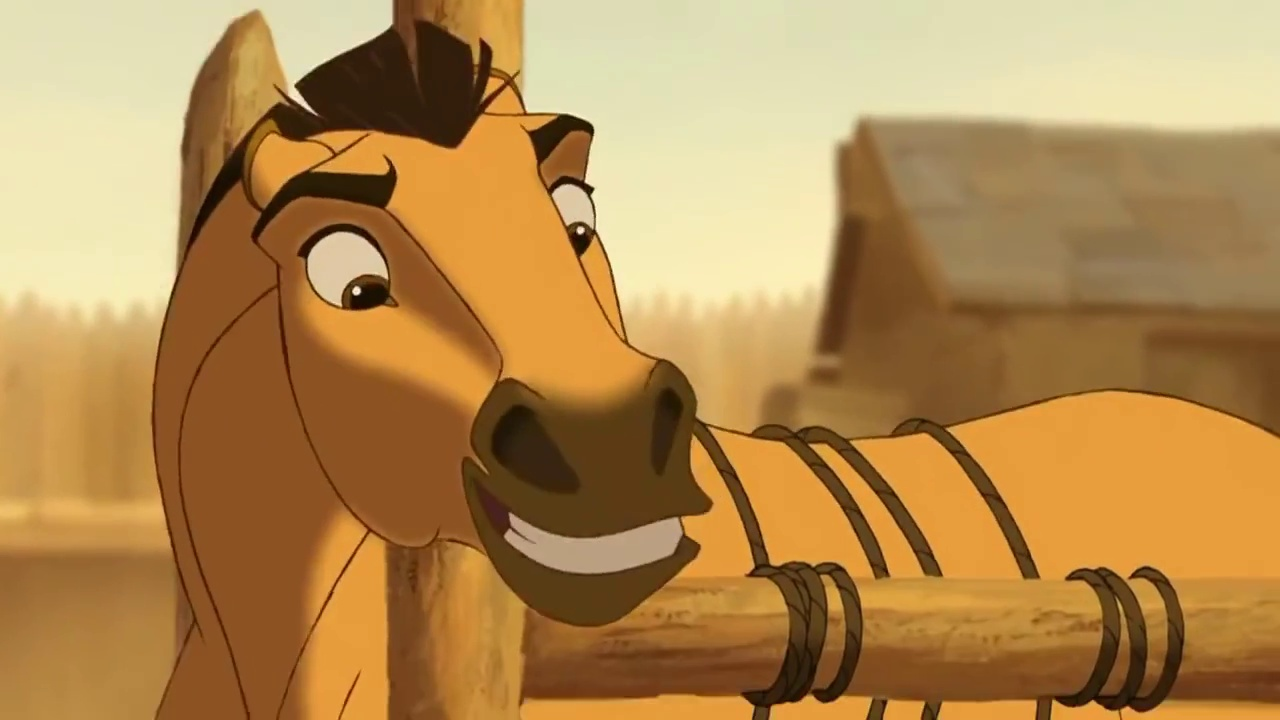
\includegraphics[width=.33\textwidth]{videoFrames/frame13.jpg}\hfill
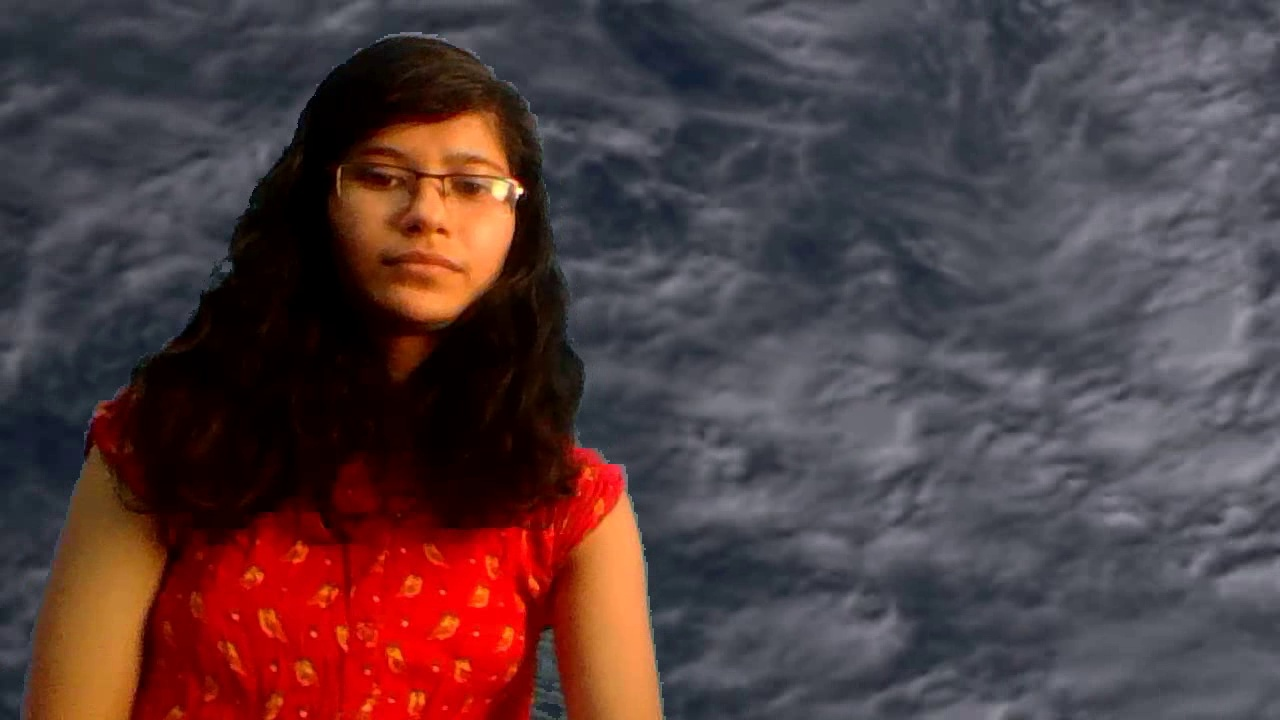
\includegraphics[width=.33\textwidth]{{videoFrames/frame14.jpg}}\hfill
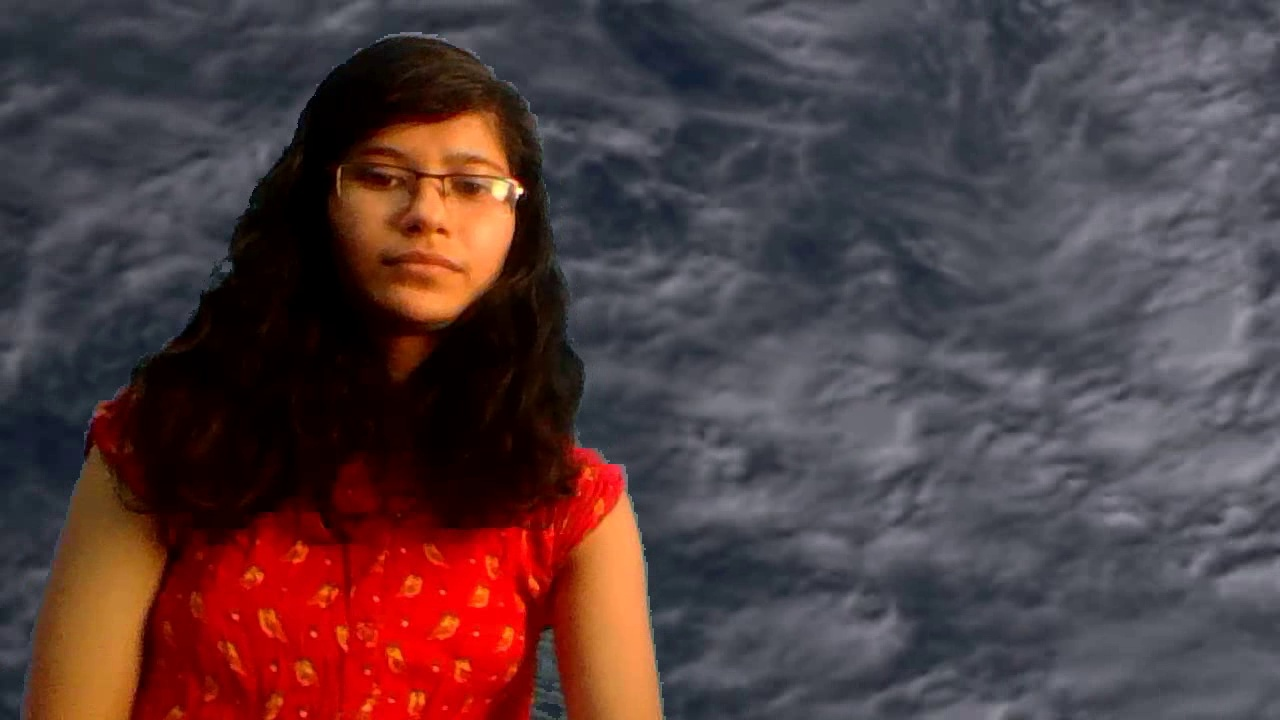
\includegraphics[width=.33\textwidth]{{videoFrames/frame15.jpg}}
\end{figure} 

 \begin{figure}[htp]
\centering

\includegraphics[width=.33\textwidth]{videoFrames/frame16.jpg}\hfill

\includegraphics[width=.33\textwidth]{{videoFrames/frame17.jpg}}\hfill
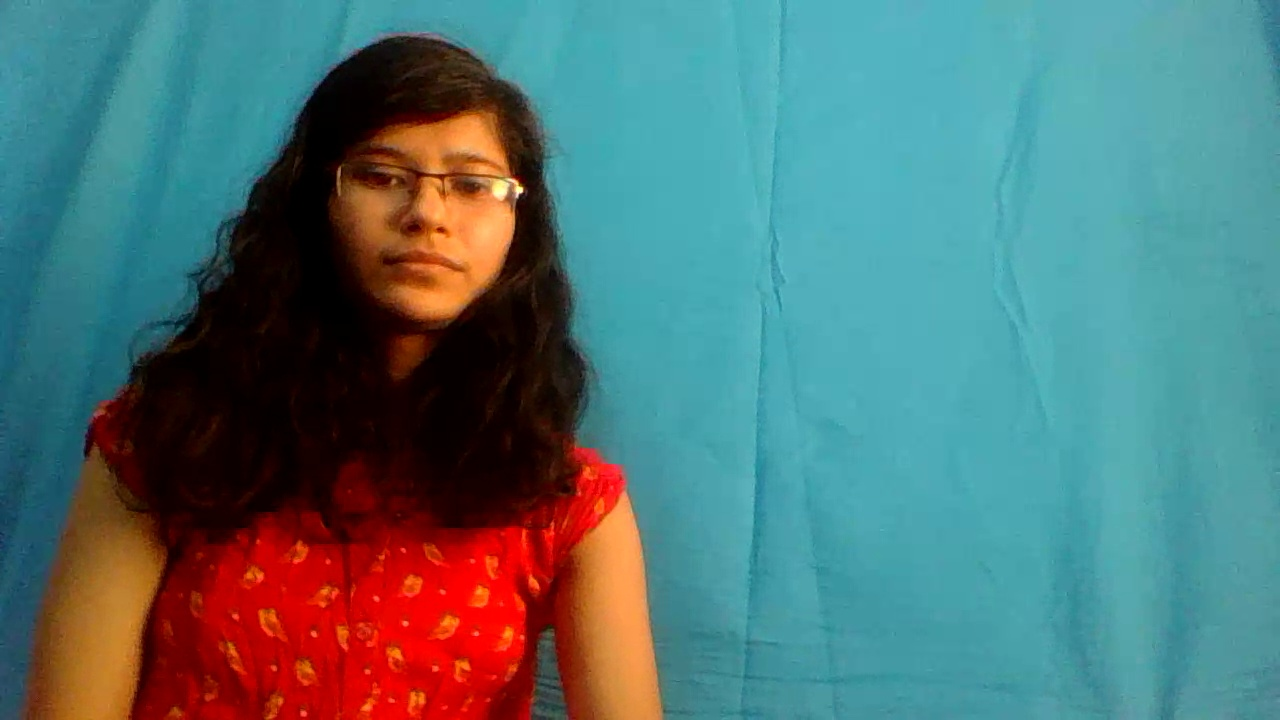
\includegraphics[width=.33\textwidth]{{videoFrames/frame18.jpg}}
\end{figure} 

\begin{figure}[htp]
\centering

\includegraphics[width=.33\textwidth]{videoFrames/frame19.jpg}\hfill
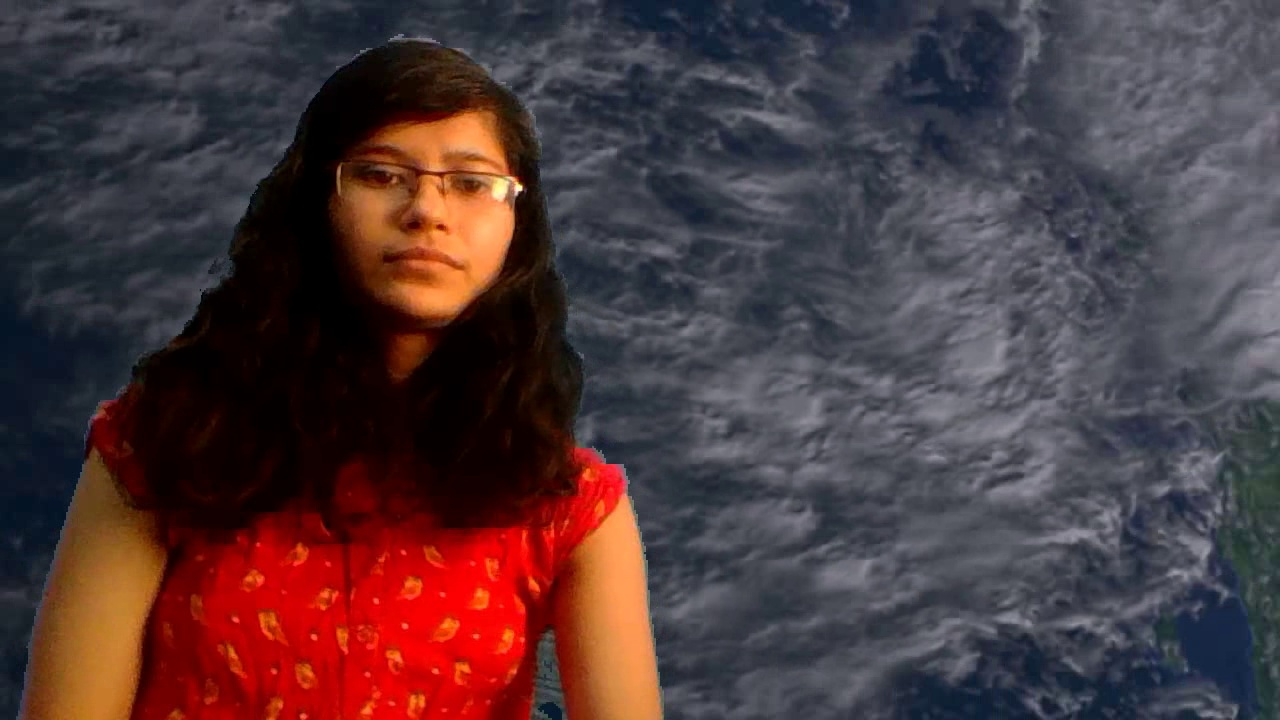
\includegraphics[width=.33\textwidth]{{videoFrames/frame20.jpg}}\hfill

\includegraphics[width=.33\textwidth]{{videoFrames/frame21.jpg}}
\end{figure} 

 \begin{figure}[htp]
\centering

\includegraphics[width=.33\textwidth]{videoFrames/frame22.jpg}\hfill
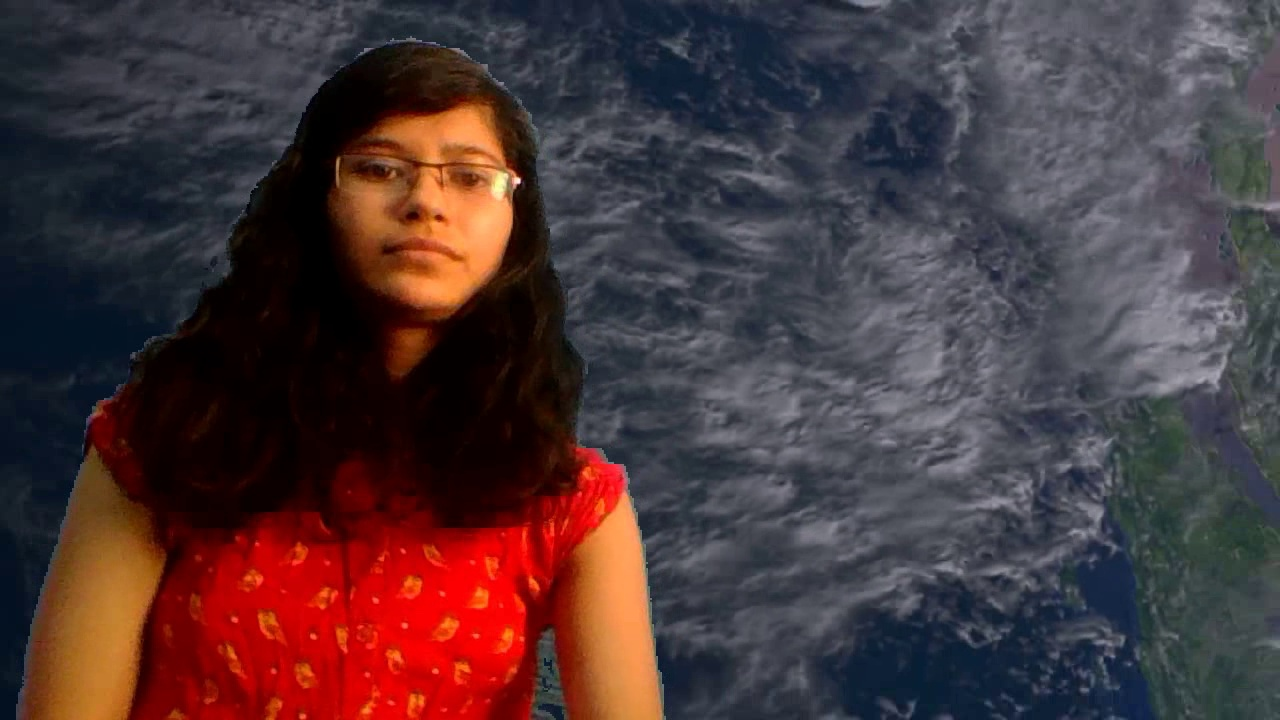
\includegraphics[width=.33\textwidth]{{videoFrames/frame23.jpg}}\hfill
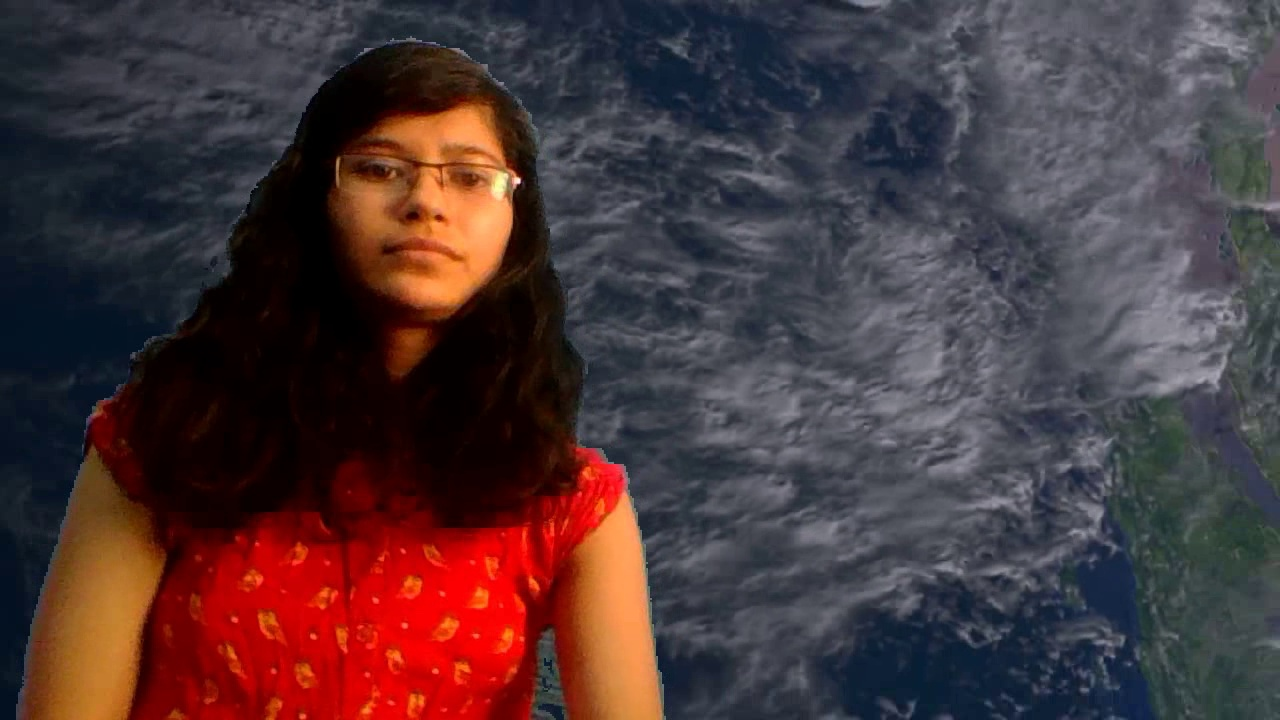
\includegraphics[width=.33\textwidth]{{videoFrames/frame24.jpg}}
\end{figure}

\clearpage 
\section{Video Creation by Merging Images}
A video comprises of the following parameters:

\begin{center}
\textbf{Frame Rate(FPS)} = \texttt{number of frames displayed/sec} \\
\textbf{Codec} = \texttt{Compression and decompression algorithm} \\
\textbf{Frame Size} = \texttt{Height and width of the frames comprising the video} \\
\end{center}

Similar to the VideoCapture, openCV has a Class for writing a video from images or frames. The VideoWriter constructor takes as arguments the filename of the video, FPS, the codec, frame size and a boolean for checking whether the video will be grayScale or color. 
\begin{verbatim}
	VideoWriter (const String &filename, int codec, double fps, Size frameSize, bool isColor=true)
	\end{verbatim}
	

\subsection{Code} 
The program takes as argument the Frame rate(FPS). The video created will lag if the frame rate is too low and will speed up(fast-forward) if the FPS is too high. The standard FPS for motion pictures is 24 FPS but for the particular video used as input to the program the FPS was 30. 

\begin{lstlisting}[language=c++]
#include<opencv2/highgui/highgui.hpp>
#include<opencv2/core/core.hpp>
#include<iostream>
#include<string>
#include<dirent.h>
#include<vector>
#include<algorithm>

using namespace std;
using namespace cv;

//comapre function for sort function
bool comp(const string& a, const  string& b) {
    string str_a,str_b;
    str_a=a.substr(5,a.length()-9);
    str_b=b.substr(5,b.length()-9);
    int int_a,int_b;
    int_a=stoi(str_a);
    int_b=stoi(str_b);
    return (int_a<=int_b)?true:false ;
}



int main(int argc, char** argv) {
    //images path
    string filepath("videoFrames");
    if(argc > 2) {
        filepath = argv[2];
        cout << "filepath " << filepath << endl;
    }

    //access image files in the directory
    DIR *dir = opendir(filepath.c_str());
    if( dir == NULL) {
        cerr << "Directory not found " << endl;
        return -1;
    }


    string imagePath;
    struct dirent *ent;
    Mat img;
    
    //parameters for the video
    int fourcc = CV_FOURCC('F', 'M', 'P', '4');
    double fps = 30;
    if (argc > 1) {
        fps = stoi(argv[1]);
    }

       string filename("myVideo_fps" + to_string((int)fps)+ ".avi");

    CvSize framesize = cvSize(1280, 720);
    if(!fourcc) {
        cerr << "codec not found" << endl;
        return -1;
    }

    //create VideoWriter object to write images to the video file
    VideoWriter wtr(filename, fourcc, fps, framesize, true);
    
    //store all image names in a vector
    vector <string> dirContent;
    while ((ent = readdir(dir)) != NULL) {

        string imgName = ent->d_name;
        if(imgName == "." || imgName == "..")
            continue;  
        dirContent.push_back(string(ent->d_name));
    }
    closedir(dir);

    //sort the images names
    sort(dirContent.begin(), dirContent.end(), comp);

    //write the images to the video 
    for(int i = 0; i < dirContent.size(); i++) {
        string imgPath =  filepath + "/" + dirContent[i];
        img = imread(imgPath);
        wtr << img;
    } 
    return 0;
}
\end{lstlisting}

\subsection{Input}
The user provides the FPS for the video to be created as a command-line argument and might optionally specify the image folder path. If no FPS is provided by the user, a default FPS of 30 is used
The input to the program are the images which were produced as output in the previous program as shown in figures \ref{figure1}.

\subsection{Output}
The output videos at various FPS can be viewed in the following folder \url{https://www.dropbox.com/sh/n5tq49i62pr31pm/AACnLS2egKQnbrv5htjepbsfa?dl=0} 

Videos with various FPS:
\begin{itemize}
\item Output video with FPS of 10 can be viewed at \url{https://www.dropbox.com/s/80vv2icy10b9tsy/myVideo_fps10.avi?dl=0} 
\item Output video with FPS of 60 can be viewed at \url{https://www.dropbox.com/s/vcutpupd0dfofmt/myVideo_fps60.avi?dl=0}
\item Output video with FPS of 30 can be viewed at \url{https://www.dropbox.com/s/otsjquty8ab0wip/myVideo_fps30.avi?dl=0}.
\end{itemize}


\section{Capturing Images from Webcam video}
Capturing video from webcam works the same way as reading a video from a file. To differentiate between the two the constructor takes as argument an integer which indicates the device number. The constructor is as follows
\begin{verbatim}
VideoCapture(int device)
\end{verbatim}

To open the default camera \texttt{VideoCapture(0)} is used. To open the current device enumerated in the system \texttt{VideoCapture(-1)} is used. To open a specific device, the index of the enumerated device has to be passed to the constructor.

\subsection{Code}
\begin{lstlisting}[language=c++]
#include<iostream>
#include<string>
#include<opencv2/core/core.hpp>
#include<opencv2/highgui/highgui.hpp>

using namespace std;
using namespace cv;

int main(int argc, char** argv) {
        //create video object from default camera
        VideoCapture cap(0);
        if(!cap.isOpened()) {
                cerr << "Camera cannot be opened" << endl;
                return -1;
        }

        //copy frames into filepath
        Mat frame;
        string filepath = "cameraFrames/";
        int num = 1;
        char c;

        //keep on recording and diplaying video until user presses 'q'
        while(c != 'q') {
                cap >> frame;
                if(!frame.data)
                        continue;
                string path = filepath + to_string(num++) + ".jpg";
                imwrite(path, frame);
                imshow("video", frame);
                c = waitKey(30);
        }
        return 0;
}
\end{lstlisting}

\subsection{Input}
The program does not take any input from the user but automatically opens the video camera connected to the system and forms the constituent images until a 'q' is pressed by the user.

\subsection{Output}
The output is the constituent frames of the webcam video. \\
All the frames for the video can be viewed at \url{https://www.dropbox.com/sh/byujjm4bxwyl5d5/AABwS1Y4jAyAjnQlt6588rhYa?dl=0}. 

A few frames of the video are as shown in the following figure \ref{webcam1}, \ref{webcam3}, \ref{webcam4}, \ref{webcam4}, \ref{webcam5}, \ref{webcam6}. 
\begin{figure}[htp]
\centering
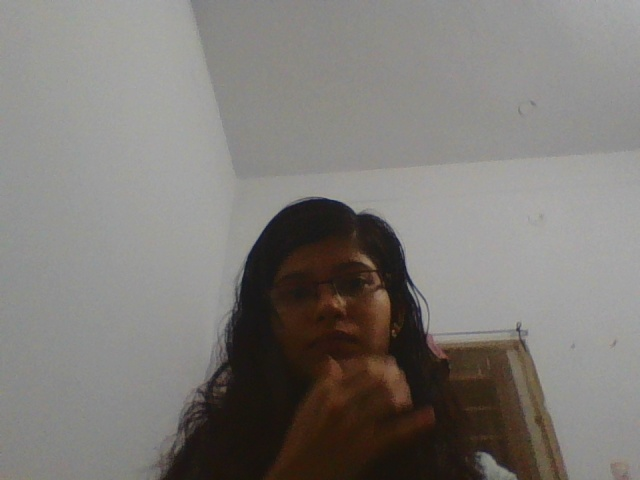
\includegraphics[width=.33\textwidth]{cameraFrames/10.jpg}\hfill
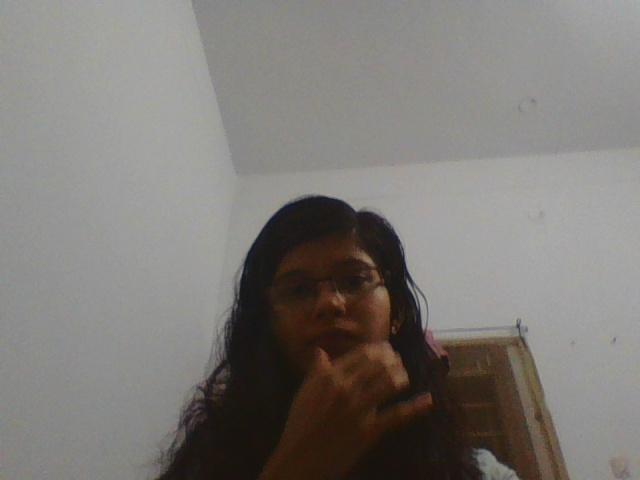
\includegraphics[width=.33\textwidth]{{cameraFrames/11.jpg}}\hfill
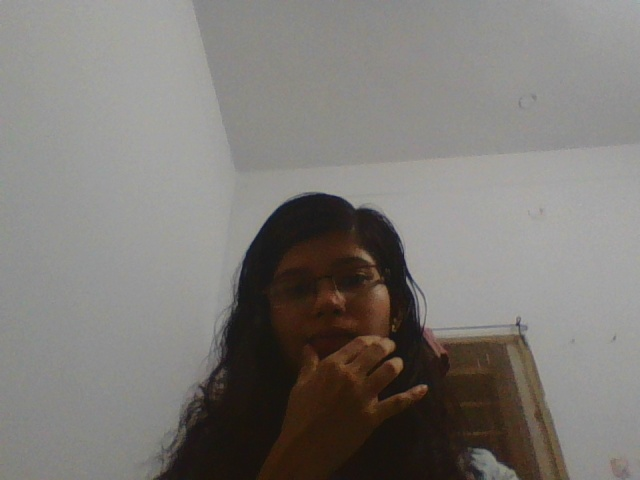
\includegraphics[width=.33\textwidth]{{cameraFrames/12.jpg}}
\end{figure}
\label{webcam1}

\begin{figure}[htp]
\centering
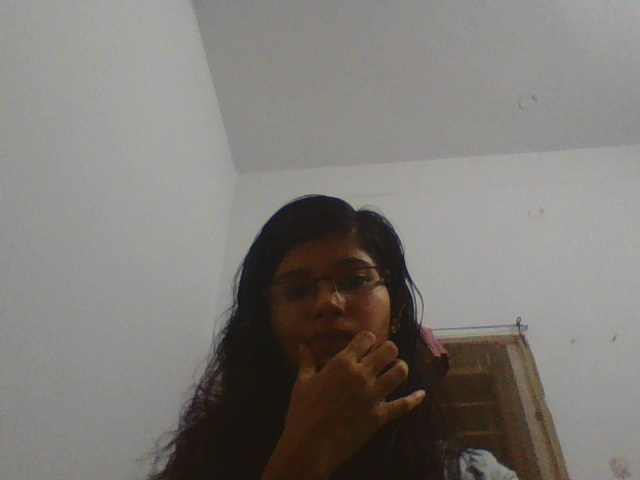
\includegraphics[width=.33\textwidth]{cameraFrames/16.jpg}\hfill
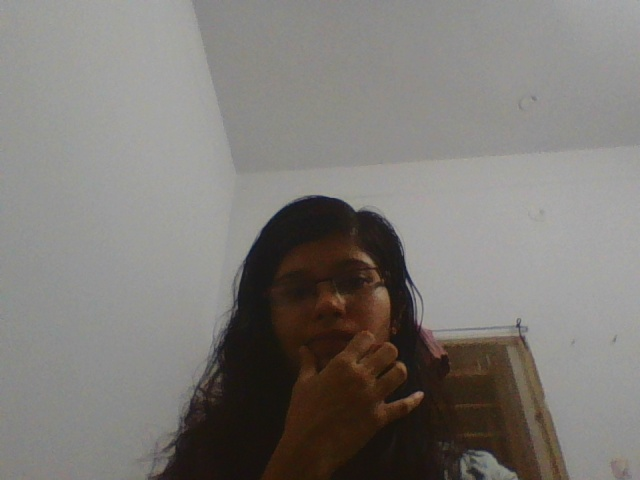
\includegraphics[width=.33\textwidth]{{cameraFrames/17.jpg}}\hfill
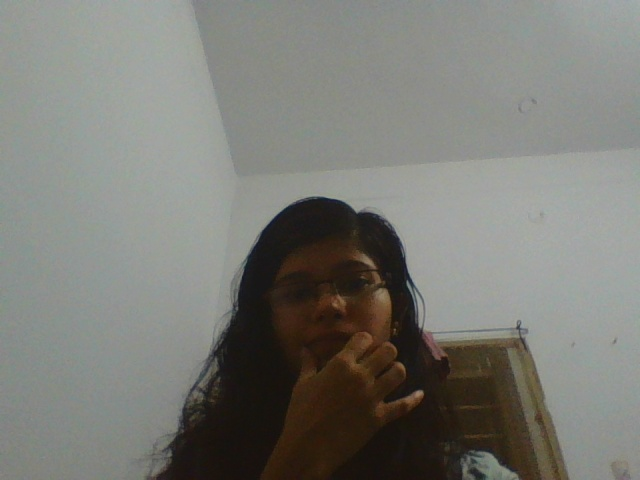
\includegraphics[width=.33\textwidth]{{cameraFrames/18.jpg}}
\end{figure} 
\label{webcam3}

\begin{figure}[htp]
\centering
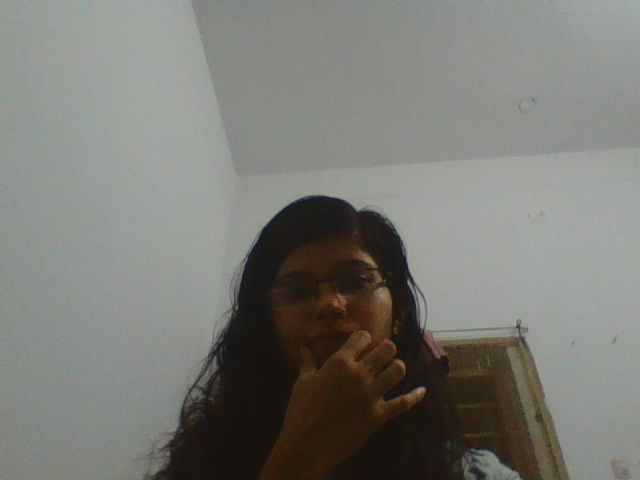
\includegraphics[width=.33\textwidth]{cameraFrames/19.jpg}\hfill
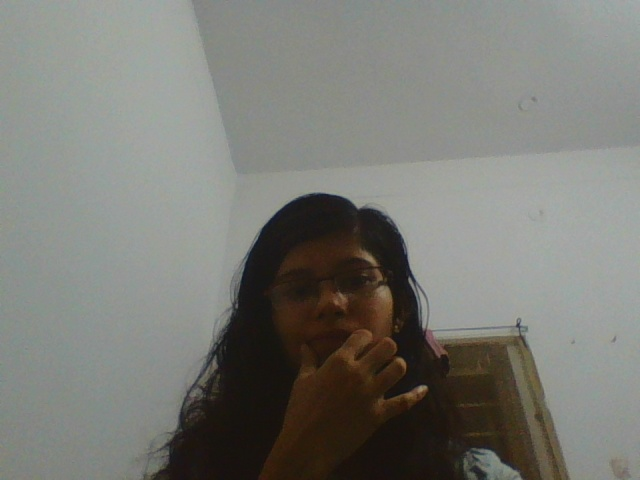
\includegraphics[width=.33\textwidth]{{cameraFrames/20.jpg}}\hfill
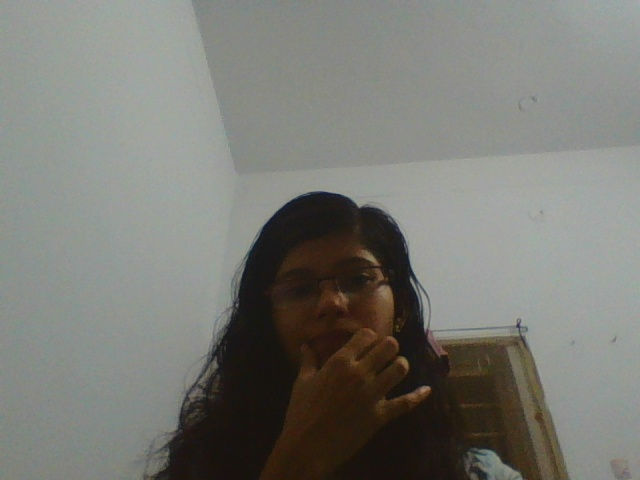
\includegraphics[width=.33\textwidth]{{cameraFrames/21.jpg}}
\end{figure} 
\label{webcam4}

 \begin{figure}[htp]
\centering
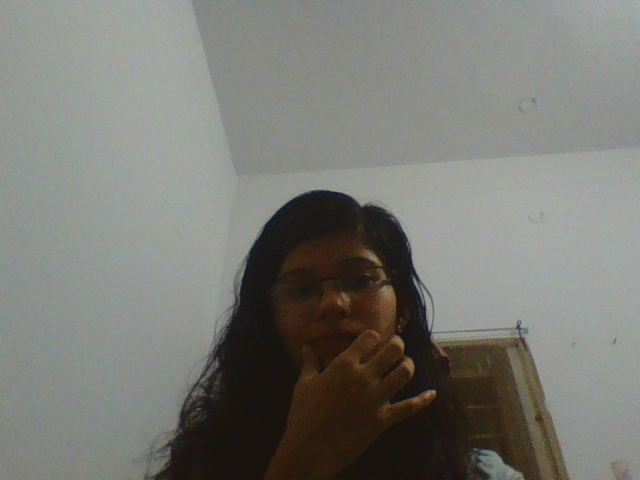
\includegraphics[width=.33\textwidth]{cameraFrames/22.jpg}\hfill
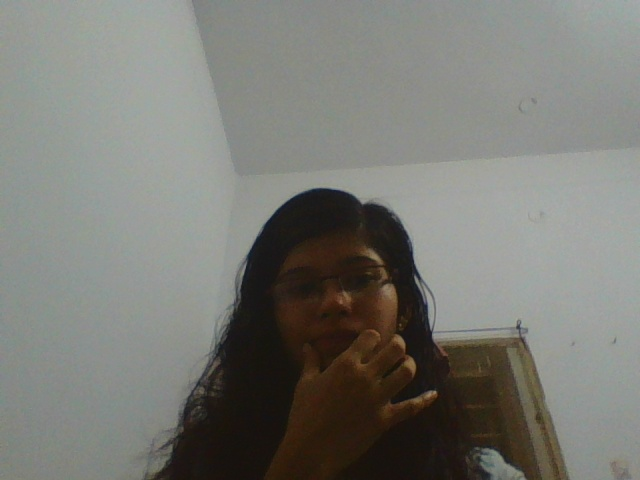
\includegraphics[width=.33\textwidth]{{cameraFrames/23.jpg}}\hfill
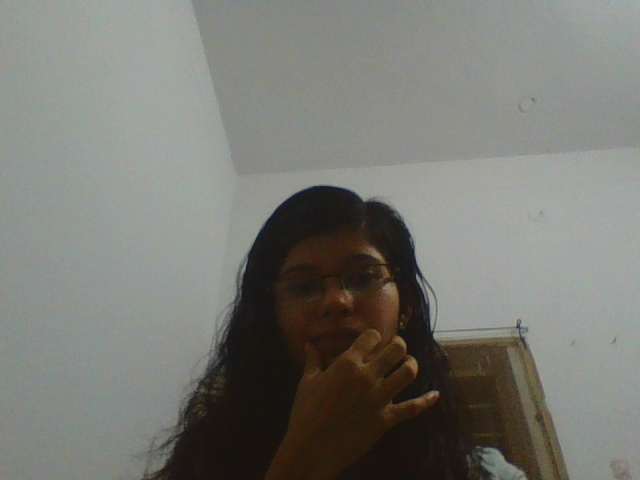
\includegraphics[width=.33\textwidth]{{cameraFrames/24.jpg}}
\end{figure}
\label{webcam5}

 \begin{figure}[htp]
\centering
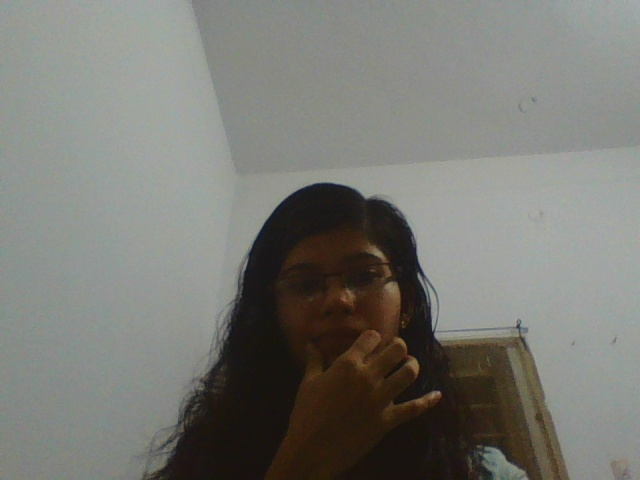
\includegraphics[width=.33\textwidth]{cameraFrames/25.jpg}\hfill
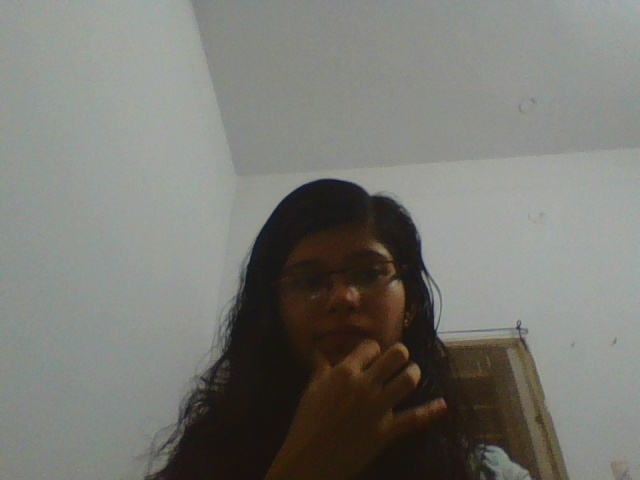
\includegraphics[width=.33\textwidth]{{cameraFrames/26.jpg}}\hfill
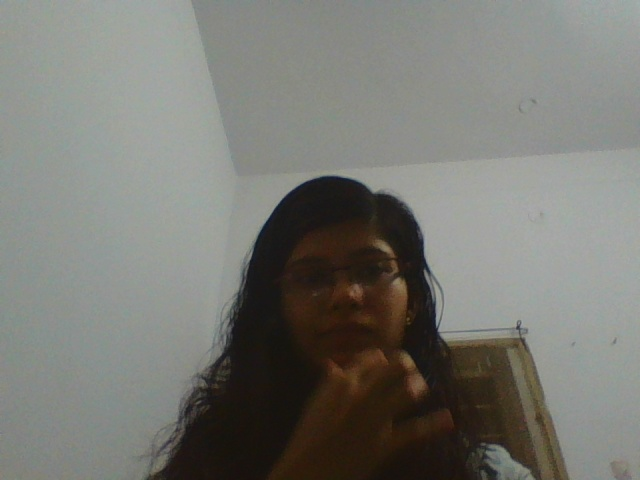
\includegraphics[width=.33\textwidth]{{cameraFrames/27.jpg}}
\end{figure}
\label{webcam6}
 
\clearpage 
\section{Chroma Keying}
Chroma keying is a technique used for combining two frames or images by replacing a color or a color range in one frame with that from the another frame. The principle behind chroma keying is that the color blue is the opposite color of skin tone, so a distinction between the two is very clear, making it easier to select the color without worrying about any part of the actor being included in the selection. The whole blue selection is then replaced with another frame as the background.

In the experiment, 2 videos are used with the background video being that of space and the foreground video of the subject. A blue backdrop is used for taking the foreground video so that the backdrop can be easily replaced with the background frame pixels.

\subsection{Procedure}
Chrominance filtering is used to replace the backdrop by the background pixels. This is used in place of RGB color intensity filtering to give better results at the edges. \\
The foreground frame is converted from RGB color space to YUV color space. This is done so that lumiance or intensity doesn't affect the thresholding. Then, the foreground frame pixels are compared against a threshold of 120, where blue is represented by a value less than 120 in the U(blue-difference) channel. \\

The output video has a frame size of the smallest input frames and FPS of the slowest video. The input frames are resized to be the size of the smallest frame.

\subsection{Code}
\begin{lstlisting}[language=c++]
#include<opencv2/core/core.hpp>
#include<opencv2/highgui/highgui.hpp>
#include<opencv2/imgproc/imgproc.hpp>
#include<iostream>
#include<string>

using namespace cv;
using namespace std;

int main(int argc, char** argv) {
   string foregrndPath("me6.webm"); 
   string backgrndPath("Fly To Space Earth.mp4");
   if(argc == 3) {
    foregrndPath = argv[1];
    backgrndPath = argv[2]; 
   }

   //foreground video object
   VideoCapture foregrndCap(foregrndPath);
   if(!foregrndCap.isOpened()) {
      cerr << "Cannot open 1st video!" << endl;
      return -1;
   }
   
   //FPS of foreground video
   double foregrndFps = foregrndCap.get(CV_CAP_PROP_FPS);

   //background video object
   VideoCapture backgrndCap(backgrndPath);
   if(!backgrndCap.isOpened()) {
      cerr << "Cannot open 2nd video!" << endl;
      return -1;
   }

   //FPS of background video
   double backgrndFps = backgrndCap.get(CV_CAP_PROP_FPS);
   
   Mat frame1, frame2;
   
   //encoding of the output video
   int fourcc = CV_FOURCC('F', 'M', 'P', '4');
   if(!fourcc) {
      cerr << "codec not found" << endl;
      return -1;
   }
      
   //FPS of output video chosen to be the smaller FPS of input videos
   double fps;
   if(foregrndFps < backgrndFps) 
      fps = foregrndFps;   
   else
      fps = backgrndFps;

   // FPS provided by user 
   if (argc > 2) {
      fps = stoi(argv[2]);
   }

   Mat foregrnd, backgrnd;
   foregrndCap >> foregrnd;
   backgrndCap >> backgrnd;
   
   //output frame size chosen to be the smaller of the input videos
   Size foreSz = foregrnd.size();
   Size backSz = backgrnd.size();
   int mergedHt = foreSz.height, mergedWdth = foreSz.width;
   if(foreSz.height > backSz.height) 
   mergedHt = backSz.height;
   if(foreSz.width > backSz.width)
    mergedWdth = backSz.width;

   CvSize framesize = cvSize(mergedWdth, mergedHt);

   // output video object creation
   VideoWriter wtr("mergedVideo.avi", fourcc, fps, framesize, true);

   // read frames from input videos until 
   // either of the 2 videos are done
   while(true) { 
      foregrndCap >> frame1;
      backgrndCap >> frame2;

      // if no more frames to read, then done
      if(frame1.empty() || frame2.empty()) {
         break;
      }

      //resize image frames to be the smallest frame size
      resize(frame1, frame1, framesize);
      resize(frame2, frame2, framesize);
      
      Mat foregrnd, backgrnd = frame2;
      Mat output(frame1.rows, frame1.cols, frame1.type());
      vector<Mat> channels;
      
      // convert foreground frame from RGB to YUV colorspace
      cvtColor(frame1, foregrnd, CV_BGR2YUV);
      
      // split the foreground frame into Y, U, V channels      
      split(foregrnd, channels);
      
      for(int y = 0; y < frame1.rows; y++) {
          for(int x = 0; x < frame1.cols; x++) {
          
          //if color blue-diff channel has value less than 120, 
          //then replace pixel val with background value
              Vec3b color = foregrnd.at<Vec3b>(Point(x,y));
                  if(color[1] > 120) {
                    output.at<Vec3b>(Point(x,y)) \ 
                     = frame1.at<Vec3b>(Point(x,y));
                  }
                  else {
                      output.at<Vec3b>(Point(x,y)) \
                      = frame2.at<Vec3b>(Point(x,y));
                  }
 
          }
      }
      //stream output frame to video object
      wtr << output;
   }
    return 0;
}
\end{lstlisting}
\subsection{Input}
The input comprises of 2 videos- one comprises of the subject with a blue backdrop and the other comprises of the background which will replace the blue backdrop.
The following are some of the frames of the foreground and backgorund videos:

A few shots of the videos are as shown in the following section.


\subsubsection{Foreground Video Frames}
The foreground video can be viewed at \url{https://www.dropbox.com/s/554mejmmfa8h1n9/me6.webm?dl=0}

A few frames of the foreground video is as follows \ref{foregrnd}
 \begin{figure}[htp]
\centering
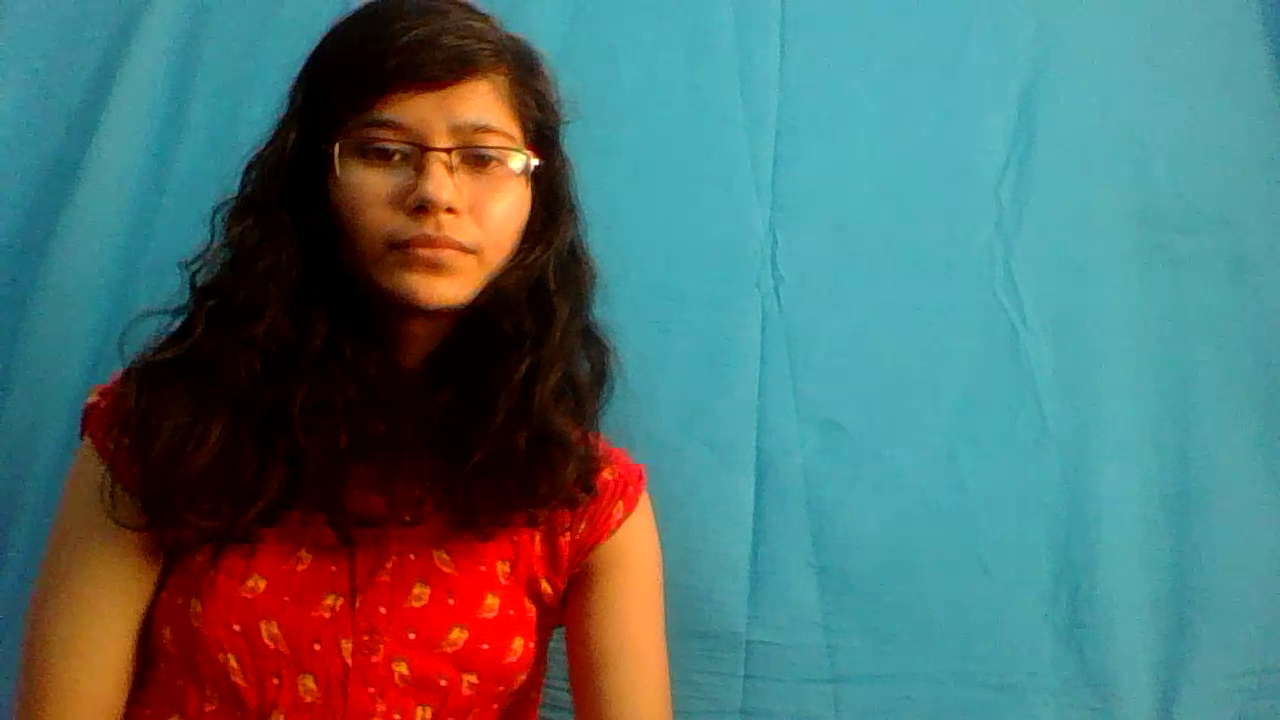
\includegraphics[width=.33\textwidth]{meOrg/frame96.jpg}\hfill
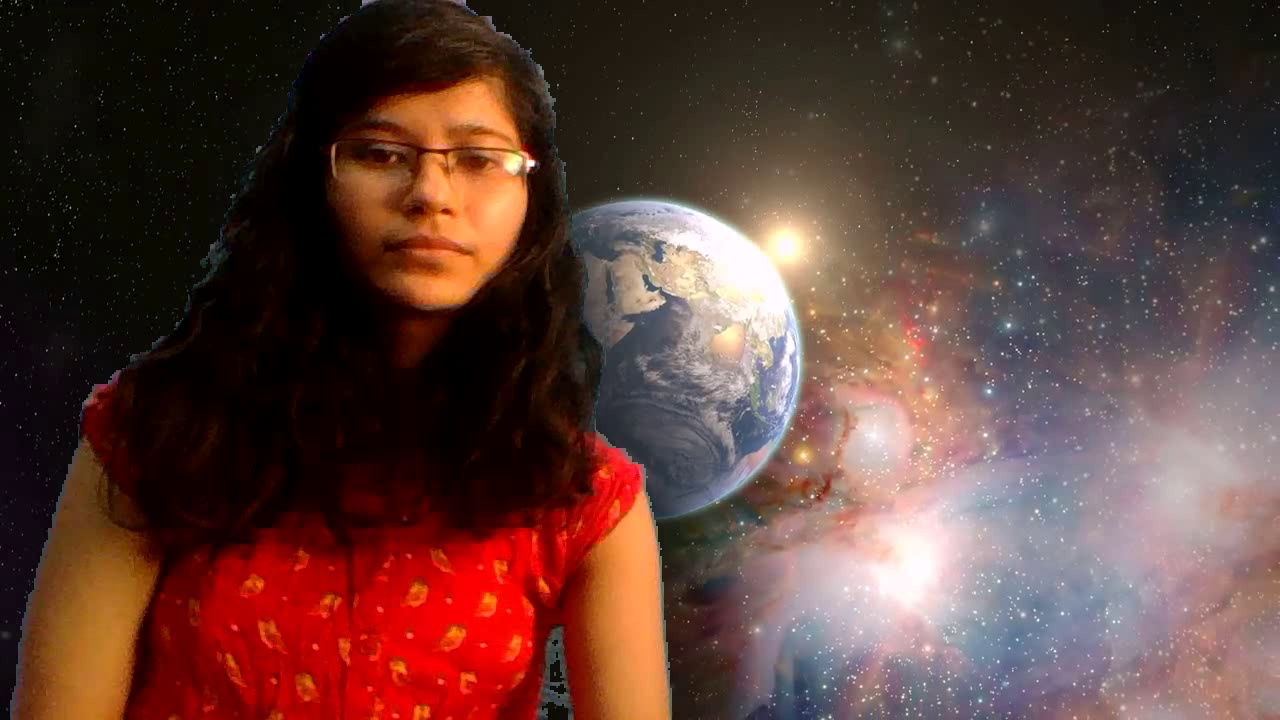
\includegraphics[width=.33\textwidth]{{meOrg/frame97.jpg}}\hfill
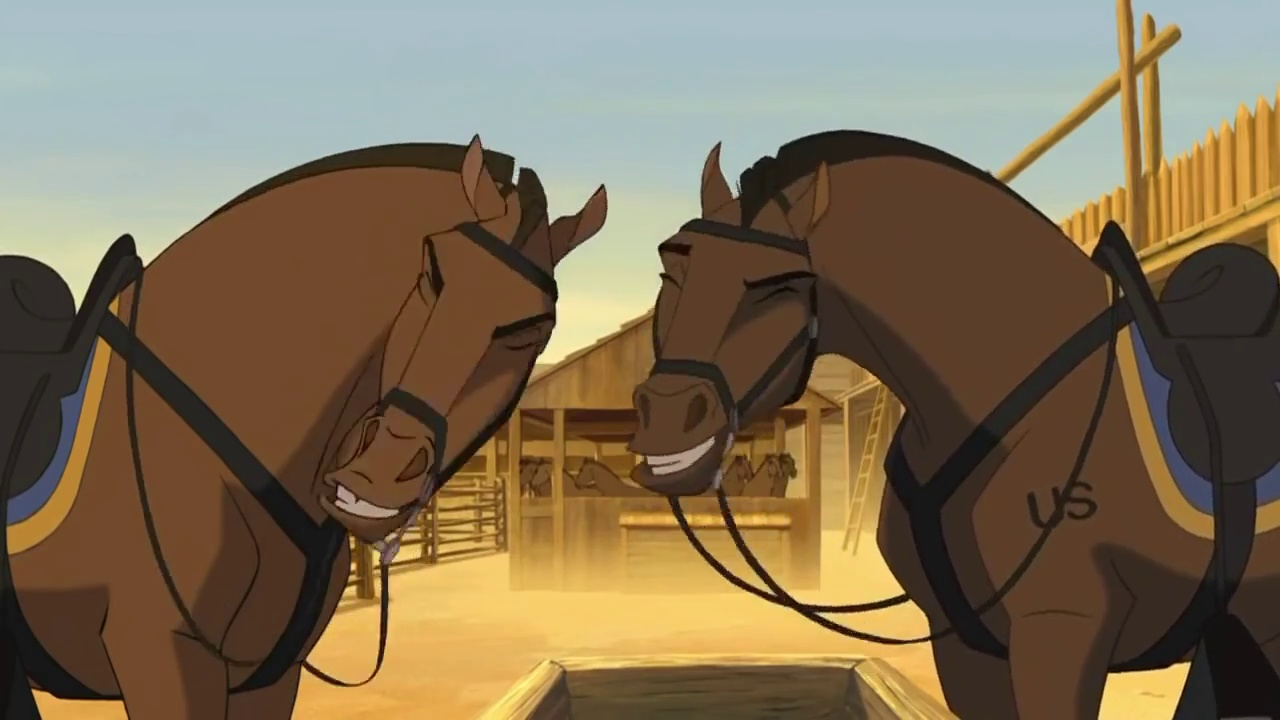
\includegraphics[width=.33\textwidth]{{meOrg/frame98.jpg}}
\end{figure}
\label{foregrnd}

\begin{figure}[htp]
\centering

\includegraphics[width=.33\textwidth]{meOrg/frame213.jpg}\hfill
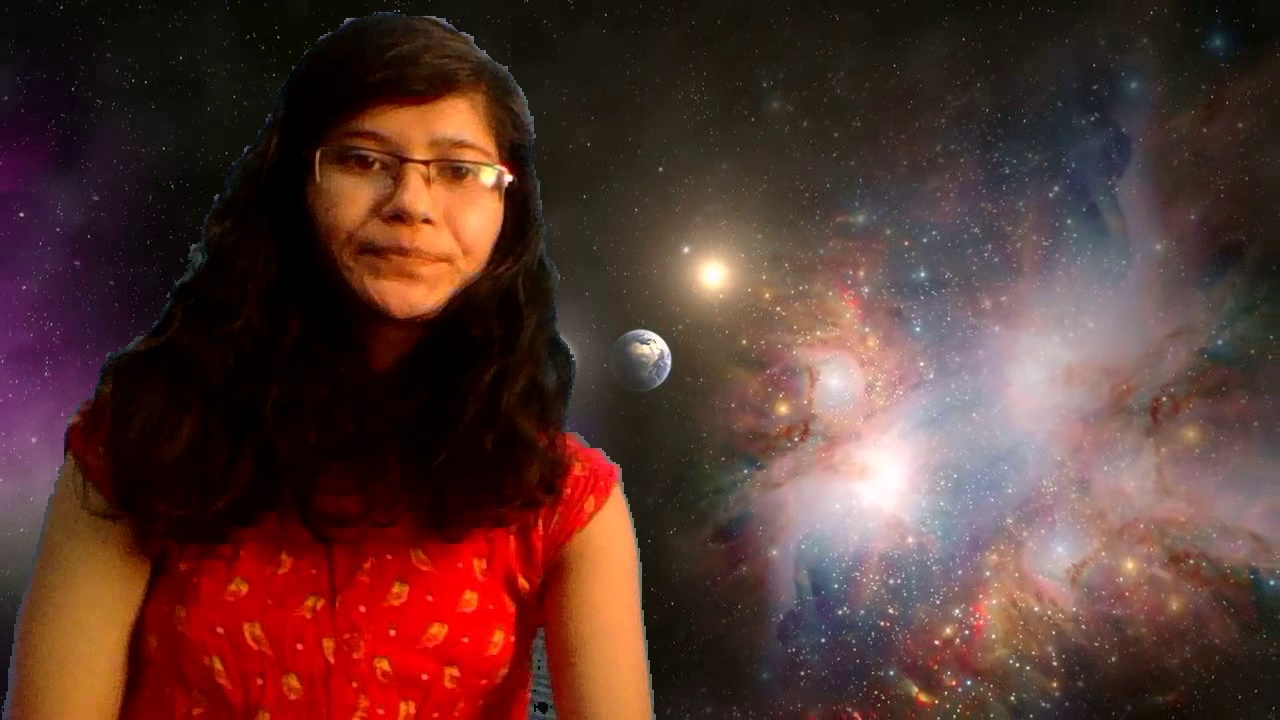
\includegraphics[width=.33\textwidth]{{meOrg/frame214.jpg}}\hfill

\includegraphics[width=.33\textwidth]{{meOrg/frame215.jpg}}
\end{figure}

 \begin{figure}[htp]
\centering

\includegraphics[width=.33\textwidth]{meOrg/frame355.jpg}\hfill

\includegraphics[width=.33\textwidth]{{meOrg/frame356.jpg}}\hfill

\includegraphics[width=.33\textwidth]{{meOrg/frame357.jpg}}
\end{figure}

\begin{figure}[htp]
\centering

\includegraphics[width=.33\textwidth]{meOrg/frame358.jpg}\hfill
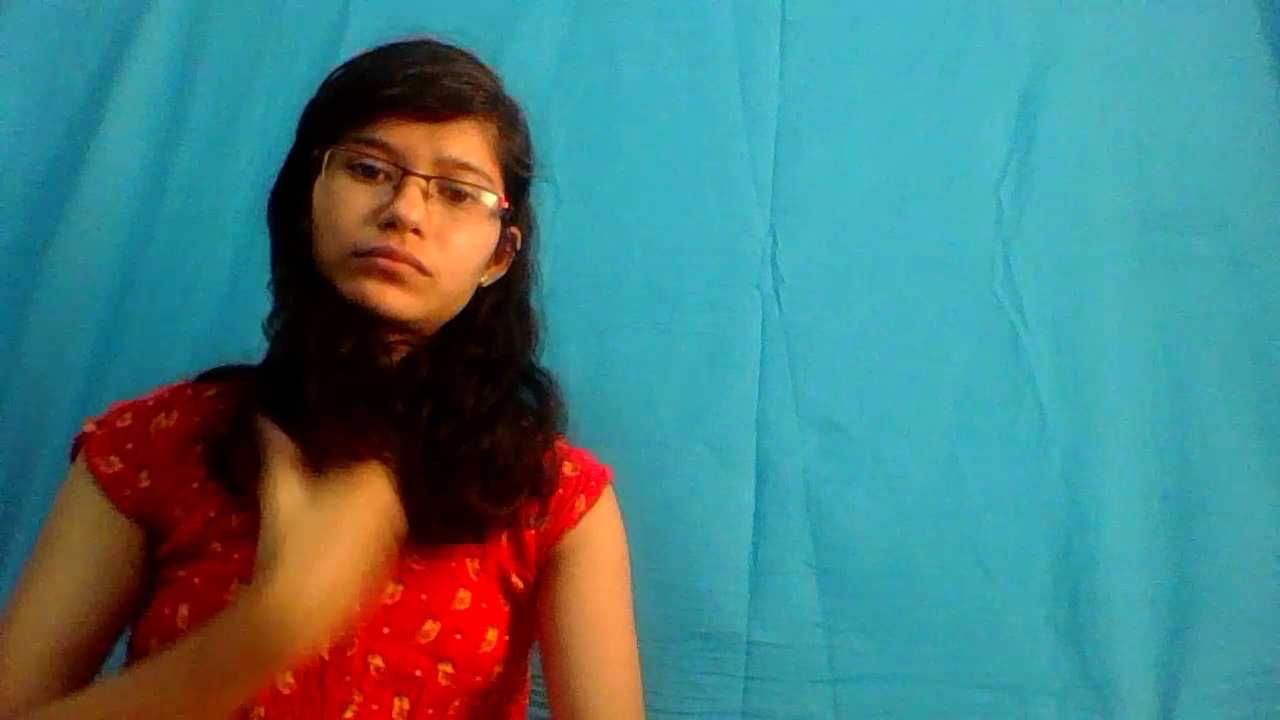
\includegraphics[width=.33\textwidth]{{meOrg/frame359.jpg}}\hfill
\includegraphics[width=.33\textwidth]{{meOrg/frame360.jpg}}
\end{figure} 


\subsubsection{Background Video Frames}
The background video can be found at \url{https://www.dropbox.com/s/k4mwule4295xyy6/Fly%20To%20Space%20Earth.mp4?dl=0}

A few frames of the background video is as follows in figures \ref{backgrnd}.

\begin{figure}[htp]
\centering
\includegraphics[width=.33\textwidth]{space/frame96.jpg}\hfill
\includegraphics[width=.33\textwidth]{{space/frame97.jpg}}\hfill
\includegraphics[width=.33\textwidth]{{space/frame98.jpg}}
\end{figure}
\label{backgrnd}

\begin{figure}[htp]
\centering
\includegraphics[width=.33\textwidth]{space/frame117.jpg}\hfill
\includegraphics[width=.33\textwidth]{{space/frame118.jpg}}\hfill
\includegraphics[width=.33\textwidth]{{space/frame119.jpg}}
\end{figure}

\begin{figure}[htp]
\centering
\includegraphics[width=.33\textwidth]{space/frame173.jpg}\hfill
\includegraphics[width=.33\textwidth]{{space/frame174.jpg}}\hfill
\includegraphics[width=.33\textwidth]{{space/frame175.jpg}}
\end{figure}

\begin{figure}[htp]
\centering
\includegraphics[width=.33\textwidth]{space/frame213.jpg}\hfill
\includegraphics[width=.33\textwidth]{{space/frame214.jpg}}\hfill
\includegraphics[width=.33\textwidth]{{space/frame215.jpg}}
\end{figure}

 \begin{figure}[htp]
\centering
\includegraphics[width=.33\textwidth]{space/frame355.jpg}\hfill
\includegraphics[width=.33\textwidth]{{space/frame356.jpg}}\hfill
\includegraphics[width=.33\textwidth]{{space/frame357.jpg}}
\end{figure}
\clearpage


\subsection{Output}
The output video for the chroma Key operation can be found at \url{https://www.dropbox.com/s/0bcpifns9p4sgxz/mergedVideo.avi?dl=0}
The output video is of the duration 17secs, ie, the smallest duration of the 2 input videos.
A 1 sec video, that has been cropped from the whole video is of the name "1.avi", is provided for reference with the submission.

A few frames of the chroma keying procedure are are shown in figures \ref{chroma1}.

 \begin{figure}[htp]
\centering
\includegraphics[width=.33\textwidth]{me/frame96.jpg}\hfill
\includegraphics[width=.33\textwidth]{{me/frame97.jpg}}\hfill
\includegraphics[width=.33\textwidth]{{me/frame98.jpg}}
\end{figure}
\label{chroma1}

\begin{figure}[htp]
\centering
\includegraphics[width=.33\textwidth]{me/frame117.jpg}\hfill
\includegraphics[width=.33\textwidth]{{me/frame118.jpg}}\hfill
\includegraphics[width=.33\textwidth]{{me/frame119.jpg}}
\end{figure}
\label{chroma2}

\begin{figure}[htp]
\centering
\includegraphics[width=.33\textwidth]{me/frame173.jpg}\hfill
\includegraphics[width=.33\textwidth]{{me/frame174.jpg}}\hfill
\includegraphics[width=.33\textwidth]{{me/frame175.jpg}}
\end{figure}
\label{chroma3}

\begin{figure}[htp]
\centering
\includegraphics[width=.33\textwidth]{me/frame213.jpg}\hfill
\includegraphics[width=.33\textwidth]{{me/frame214.jpg}}\hfill
\includegraphics[width=.33\textwidth]{{me/frame215.jpg}}
\end{figure}
\label{chroma4}

 \begin{figure}[htp]
\centering
\includegraphics[width=.33\textwidth]{me/frame355.jpg}\hfill
\includegraphics[width=.33\textwidth]{{me/frame356.jpg}}\hfill
\includegraphics[width=.33\textwidth]{{me/frame357.jpg}}
\end{figure}
\label{chroma5}

\begin{figure}[htp]
\centering
\includegraphics[width=.33\textwidth]{me/frame358.jpg}\hfill
\includegraphics[width=.33\textwidth]{{me/frame359.jpg}}\hfill
\includegraphics[width=.33\textwidth]{{me/frame360.jpg}}
\end{figure} 
\label{chroma6}

\end{document}
